\documentclass[border=4pt]{standalone}
% Shared typography and colours for the standalone figures.
\usepackage{unicode-math}
\setmainfont{TeX Gyre Termes}
\setsansfont{TeX Gyre Heros}
\setmonofont{TeX Gyre Cursor}
\setmathfont{TeX Gyre Termes Math}
\usepackage{tikz}
\usetikzlibrary{arrows.meta,positioning,calc,decorations.pathreplacing}
\usepackage{pgfplots}
\pgfplotsset{compat=1.18}
\definecolor{elemA}{HTML}{1F5FA8}
\definecolor{elemB}{HTML}{B8461B}
\definecolor{elemC}{HTML}{2E7D32}
\definecolor{elemD}{HTML}{6A4C93}
\definecolor{frameline}{HTML}{555555}

\begin{document}
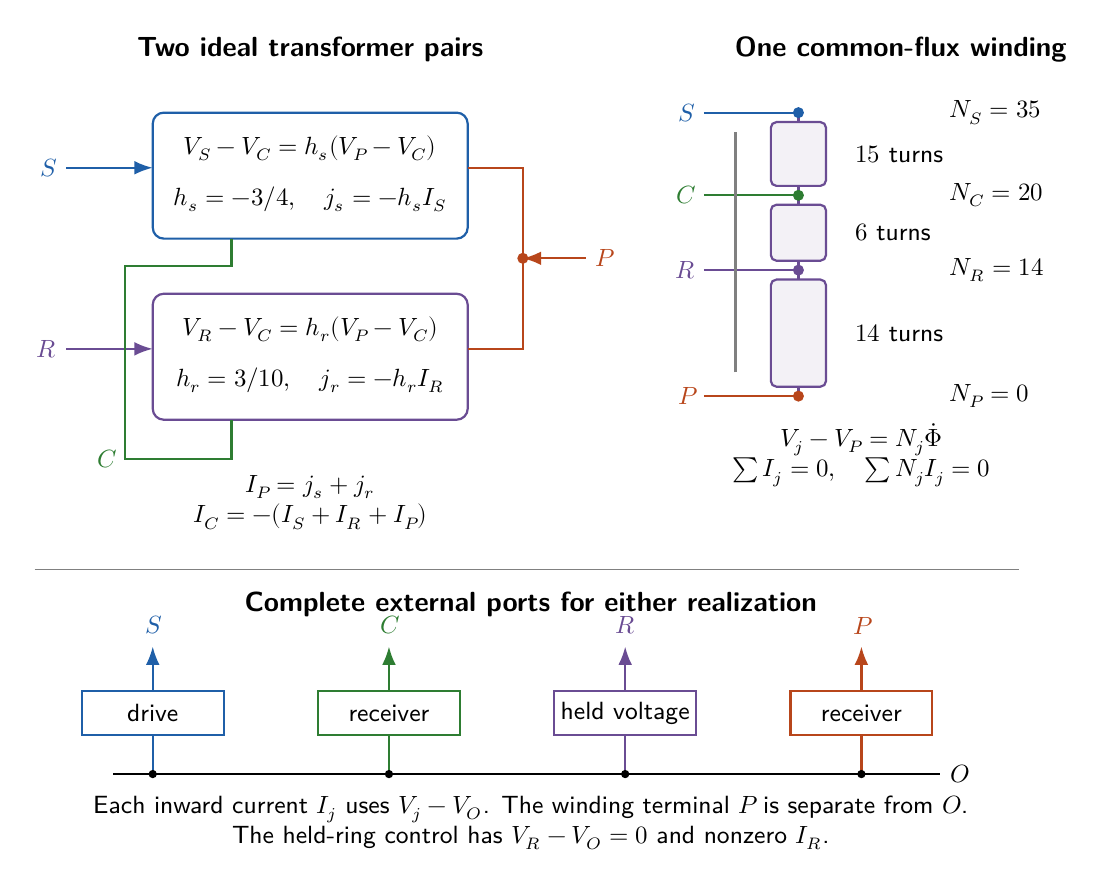
\begin{tikzpicture}[font=\sffamily\small,>=Latex]
\node[font=\sffamily\bfseries] at (3,4.6) {Two ideal transformer pairs};
\node[font=\sffamily\bfseries] at (10.5,4.6) {One common-flux winding};
\draw[elemA,thick,rounded corners] (1,2.2) rectangle (5,3.8);
\node at (3,3.35) {$V_S-V_C=h_s(V_P-V_C)$};
\node at (3,2.7) {$h_s=-3/4,\quad j_s=-h_s I_S$};
\draw[elemD,thick,rounded corners] (1,-.1) rectangle (5,1.5);
\node at (3,1.05) {$V_R-V_C=h_r(V_P-V_C)$};
\node at (3,.4) {$h_r=3/10,\quad j_r=-h_r I_R$};
\draw[->,elemA,thick] (-.1,3.1)--(1,3.1) node[pos=0,left] {$S$};
\draw[->,elemD,thick] (-.1,.8)--(1,.8) node[pos=0,left] {$R$};
\draw[elemB,thick] (5,3.1)--(5.7,3.1)--(5.7,.8)--(5,.8);
\draw[->,elemB,thick] (6.5,1.95)--(5.7,1.95);
\node[elemB,right] at (6.5,1.95) {$P$};
\fill[elemB] (5.7,1.95) circle (2pt);
\draw[elemC,thick] (2,2.2)--(2,1.85)--(.65,1.85)--(.65,-.6)--(2,-.6)--(2,-.1);
\node[elemC,left] at (.65,-.6) {$C$};
\node[align=center] at (3,-1.15) {$I_P=j_s+j_r$\\$I_C=-(I_S+I_R+I_P)$};
% A tapped winding drawn as three magnetic section blocks.
\foreach \ya/\yb/\n in {3.8/2.75/15,2.75/1.8/6,1.8/.2/14}{
 \draw[elemD,thick] (9.2,\ya)--(9.2,\yb);
 \draw[fill=elemD!8,draw=elemD,thick,rounded corners=2pt] (8.85,\yb+.12) rectangle (9.55,\ya-.12);
 \node[anchor=west] at (9.8,{(\ya+\yb)/2}) {$\n$ turns};
}
\foreach \y/\name/\turn/\col in {3.8/S/35/elemA,2.75/C/20/elemC,1.8/R/14/elemD,.2/P/0/elemB}{
 \draw[\col,thick] (8.0,\y)--(9.2,\y);
 \fill[\col] (9.2,\y) circle (2pt);
 \node[\col,left] at (8,\y) {$\name$};
 \node[right] at (11,\y) {$N_{\name}=\turn$};
}
\draw[gray,very thick] (8.4,.5)--(8.4,3.55);
\node[align=center] at (10,-.55) {$V_j-V_P=N_j\dot\Phi$\\$\sum I_j=0,\quad\sum N_jI_j=0$};
\draw[gray] (-.5,-2)--(12,-2);
\node[font=\sffamily\bfseries] at (5.8,-2.45) {Complete external ports for either realization};
\foreach \x/\n/\col/\label in {1/S/elemA/drive,4/C/elemC/receiver,7/R/elemD/held voltage,10/P/elemB/receiver}{
 \node[\col,above] at (\x,-2.95) {$\n$};
 \draw[\col,->,thick] (\x,-3.55)--(\x,-2.98);
 \draw[\col,fill=white,thick] (\x-.9,-4.1) rectangle (\x+.9,-3.55);
 \node at (\x,-3.825) {\label};
 \draw[\col,thick] (\x,-4.1)--(\x,-4.6);
 \fill (\x,-4.6) circle (1.5pt);
}
\draw[thick] (.5,-4.6)--(11,-4.6) node[right] {$O$};
\node[align=center] at (5.8,-5.22)
 {Each inward current $I_j$ uses $V_j-V_O$. The winding terminal $P$ is separate from $O$.\\
 The held-ring control has $V_R-V_O=0$ and nonzero $I_R$.};
\end{tikzpicture}
\end{document}
